\chapter{Introduction} \label{chap:Introduction}

\blindtext

\begin{figure}
    \centering
    \begin{adjustbox}{minipage=\dimexpr\textwidth-2\fboxsep-2\fboxrule,fbox}
        \begin{subfigure}[b]{0.475\textwidth}
            \caption[\textit{Alphainfluenzavirus}]{\textbf{\textit{Alphainfluenzavirus}}}
            \label{subfig:Influenza_A}
            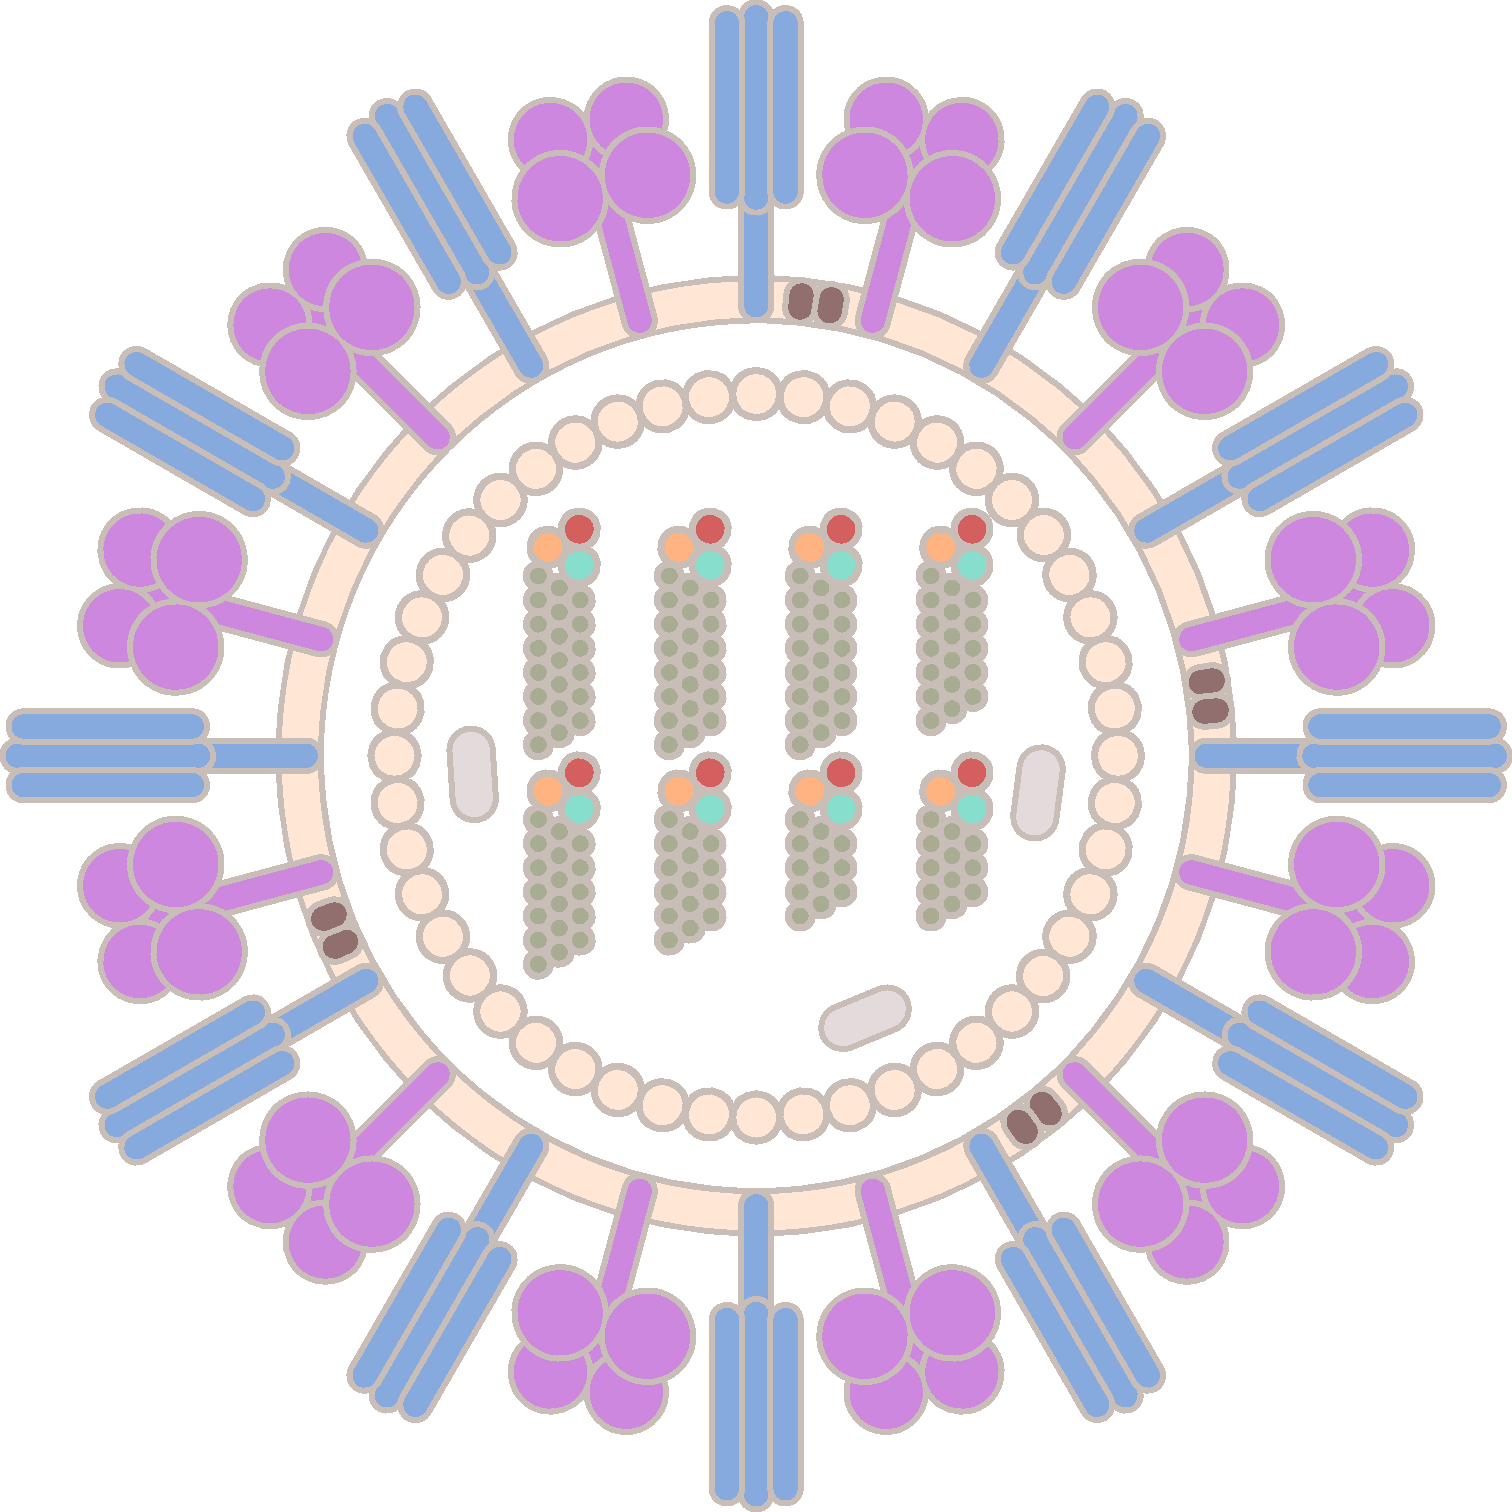
\includegraphics[width=\textwidth]{Graphics/Influenza_A.pdf}
        \end{subfigure}
        \hfill
        \begin{subfigure}[b]{0.475\textwidth}
            \caption[\textit{Betainfluenzavirus}]{\textbf{\textit{Betainfluenzavirus}}}
            \label{subfig:Influenza_B}
            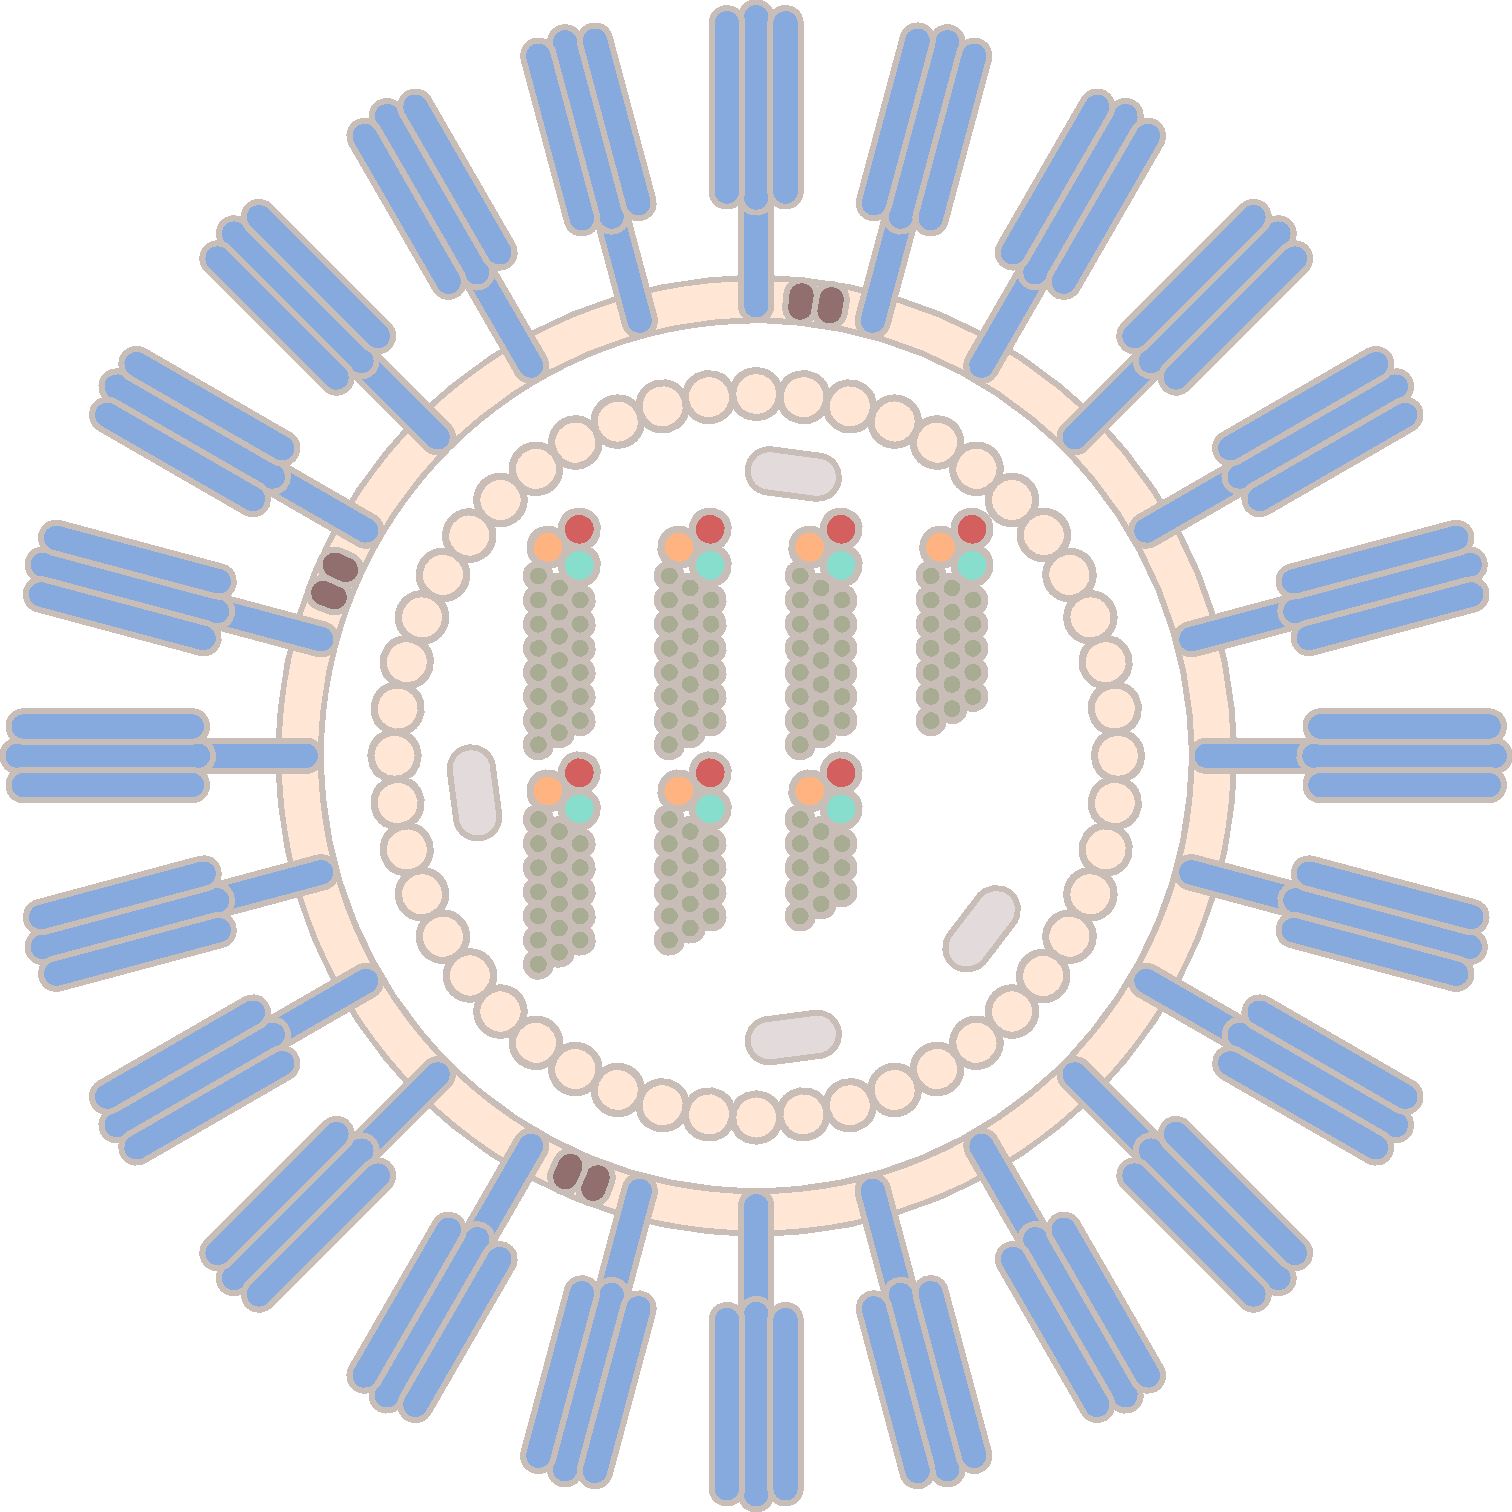
\includegraphics[width=\textwidth]{Graphics/Influenza_B.pdf}
        \end{subfigure}
    \end{adjustbox}
    \caption[\textit{Orthomyxoviridae}]{\textbf{\textit{Orthomyxoviridae}.} .}
    \label{fig:Orthomyxoviridae}
\end{figure}

\blindtext

\begin{figure}
    \centering
    \begin{adjustbox}{minipage=\dimexpr\textwidth-2\fboxsep-2\fboxrule,fbox}
        \begin{subfigure}[b]{0.475\textwidth}
            \caption[Compactness]{\textbf{Compactness}}
            \label{subfig:Compactness}            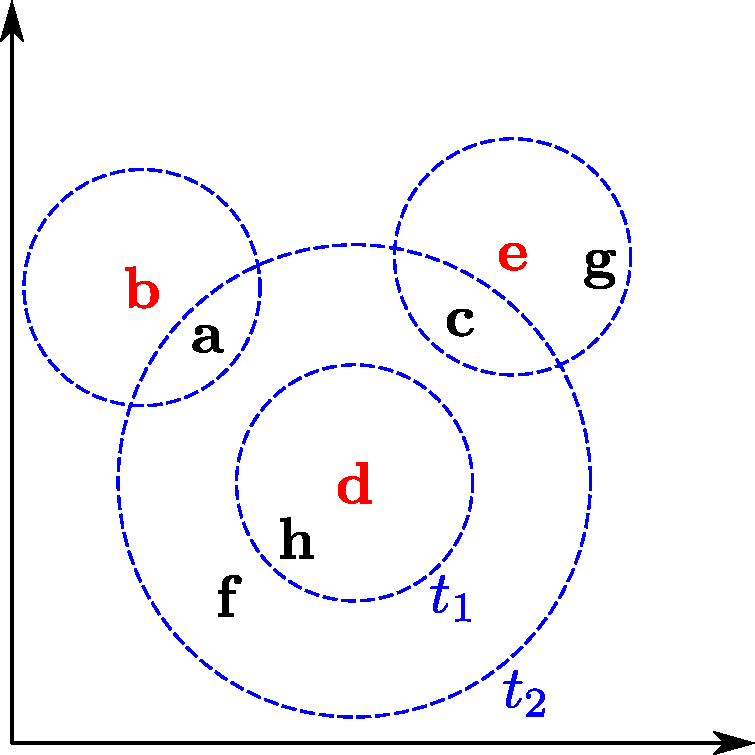
\includegraphics[width=\textwidth]{Graphics/Compactness.pdf}
        \end{subfigure}
        \hfill
        \begin{subfigure}[b]{0.475\textwidth}
            \caption[Connectedness]{\textbf{Connectedness}}
            \label{subfig:Connectedness}            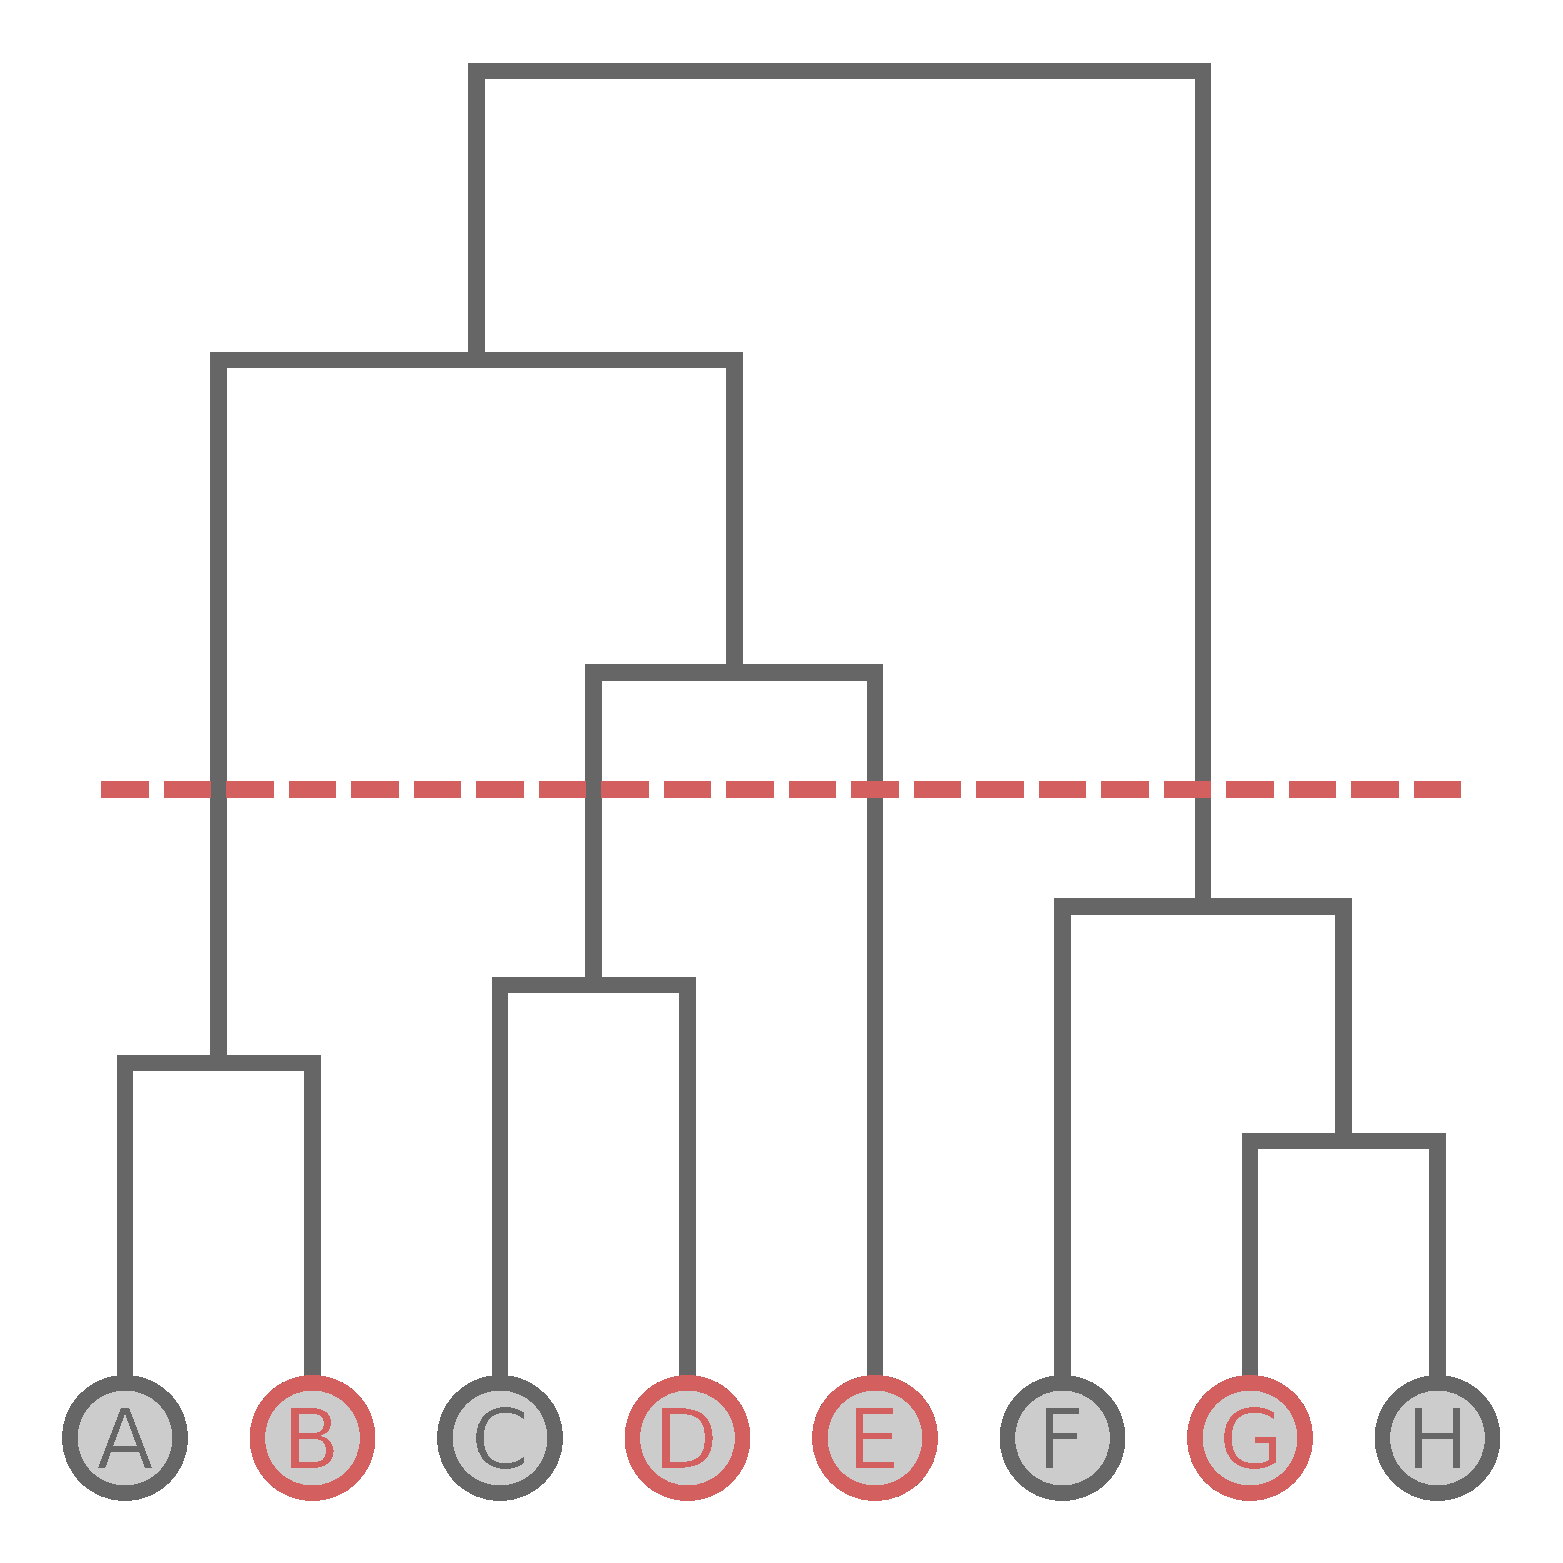
\includegraphics[width=\textwidth]{Graphics/Connectedness.pdf}
        \end{subfigure}
    \end{adjustbox}
    \caption[Clustering Methods]{\textbf{Clustering Methods.} .}
    \label{fig:Methods}
\end{figure}

\blindtext

\begin{figure}
    \centering
    \begin{adjustbox}{minipage=\dimexpr\textwidth-2\fboxsep-2\fboxrule,fbox}
        \begin{subfigure}[b]{0.475\textwidth}
            \caption[Euclidean]{\textbf{Euclidean}}
            \label{subfig:Euclidean}
            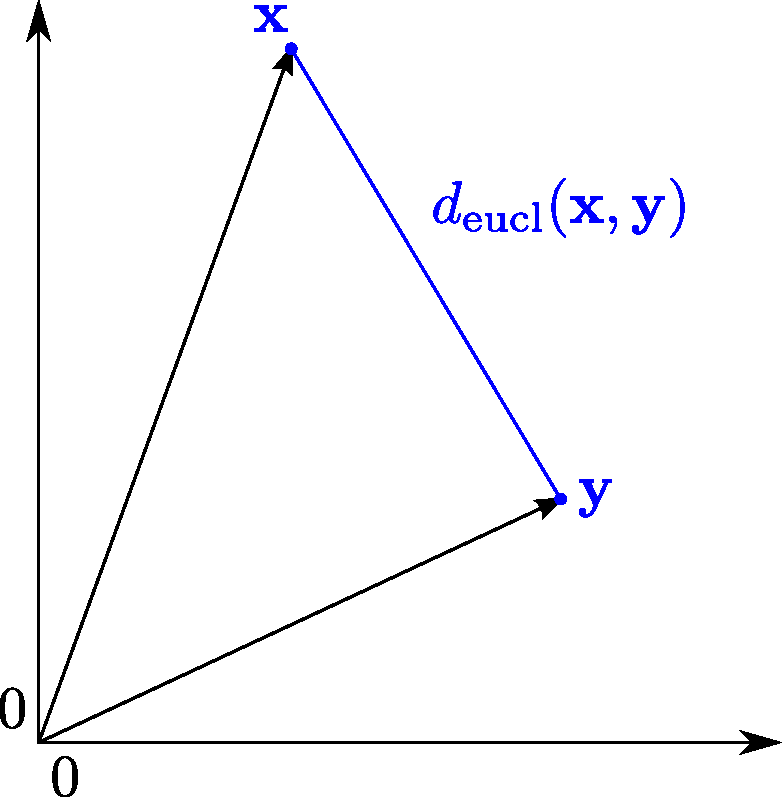
\includegraphics[width=\textwidth]{Graphics/Euclidean.pdf}
        \end{subfigure}
        \hfill
        \begin{subfigure}[b]{0.475\textwidth}
            \caption[Cosine]{\textbf{Cosine}}
            \label{subfig:Cosinus}            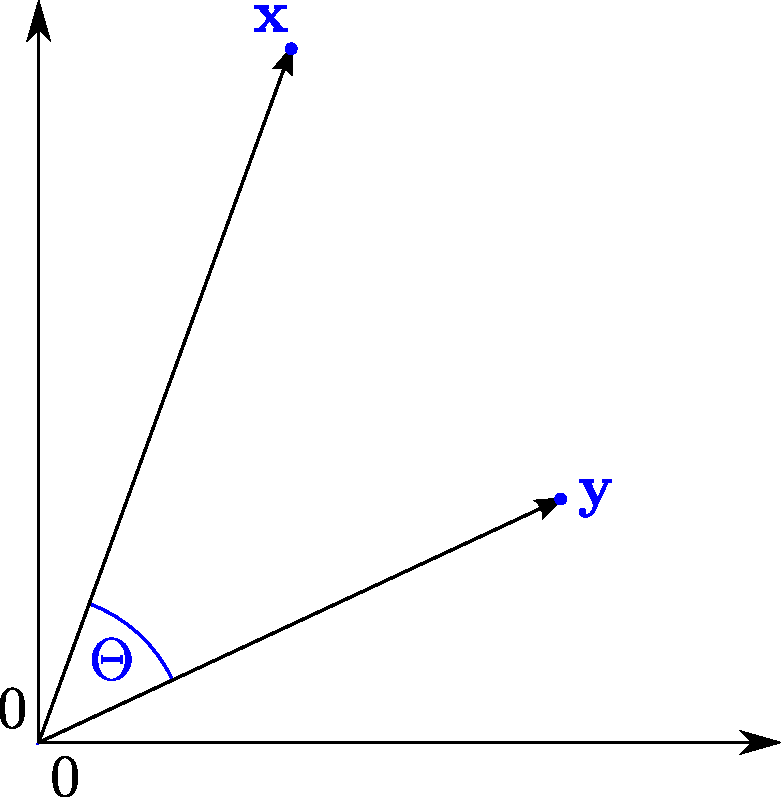
\includegraphics[width=\textwidth]{Graphics/Cosinus.pdf}
        \end{subfigure}
    \end{adjustbox}
    \caption[Distance Measuring Methods]{\textbf{Distance Measuring Methods.} .}
    \label{fig:Distance}
\end{figure}

\begin{figure}[!hbt]
    \centering
    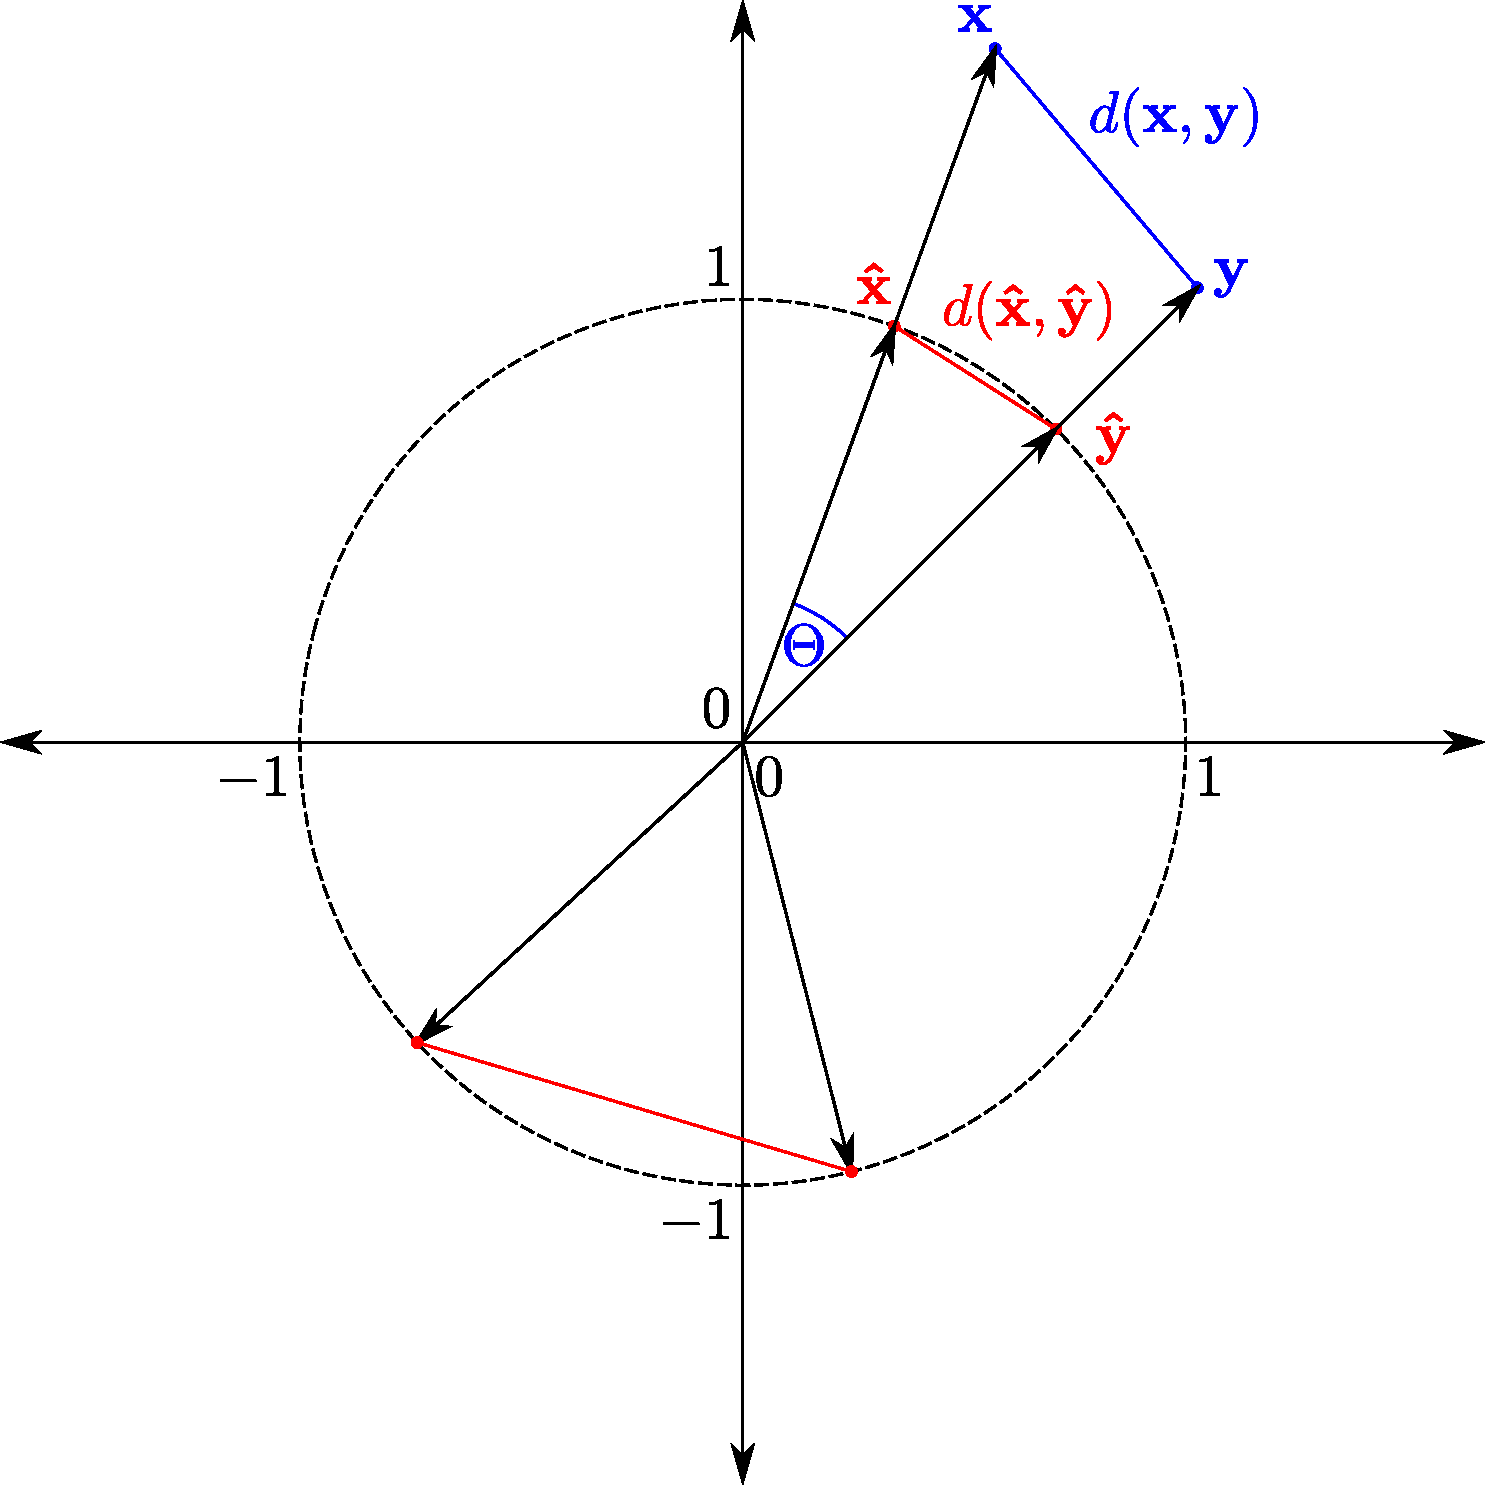
\includegraphics[width=\dimexpr\textwidth-2\fboxsep-2\fboxrule,fbox]{Graphics/L2_Euclidean.pdf}
    \caption[Mathematical Background of L2 Normalisation]{\textbf{Mathematical Background of L2 Normalisation.} .}
    \label{fig:L2_Normalisation_Background}
\end{figure}

\blindtext

% \begin{fequation}[!hbt]
%     \begin{empheq}[box=\fbox]{alignat* = -1}
%         &xL &&&&+zL &&\longrightarrow xL &&&&+zH\\
%         &xM &&+yL &&+zH &&\longrightarrow xM &&+yL &&+zL\\
%         &xM &&+yM &&+zL &&\longrightarrow xM &&+yM &&+zH\\
%         &xH &&+yL &&+zH &&\longrightarrow xH &&+yL &&+zL\\
%         &xH &&+yM &&+zH &&\longrightarrow xH &&+yM &&+zL\\
%         & &&\hphantom{++}yH &&+zL &&\longrightarrow &&\hphantom{++}yH &&+zH
%     \end{empheq}
%     \caption[]{\textbf{.}}
%     \label{gl:8.2}
% \end{fequation}

\textbf{Normalization with max-norm:} 
%is the normalization so that the l2 norm of a vector is 1 !!!!!

\begin{empheq}{alignat = -1}
    \hat{\mathbf{x}} &= \frac{\mathbf{x}}{\Vert\mathbf{x}\Vert_{\text{max}}}
\end{empheq}

\begin{empheq}{alignat = -1}
    \Vert\hat{\mathbf{x}}\Vert_{\text{max}} &= 1
\end{empheq}

\textbf{normalization with l1 norm:} 
%is the normalization so that the l2 norm of a vector is 1 !!!!!

\begin{empheq}{alignat = -1}
    \hat{\mathbf{x}} &= \frac{\mathbf{x}}{\Vert\mathbf{x}\Vert_1}
\end{empheq}

\begin{empheq}{alignat = -1}
    \Vert\hat{\mathbf{x}}\Vert_1 &= 1
\end{empheq}

\textbf{Cosinus similarity:}

\begin{empheq}{alignat = -1}
    &\cos\angle(\mathbf{x}, \mathbf{y}) &&= \frac{\mathbf{x}^\top\mathbf{y}}{\Vert\mathbf{x}\Vert \cdot \Vert\mathbf{y}\Vert}
\end{empheq}

\textbf{cosinus distance}

\begin{empheq}{alignat = -1}
    &d(\mathbf{x},\mathbf{y}) &&= 1 - \cos\angle(\mathbf{x}, \mathbf{y})
\end{empheq}

\textbf{Normalization with l2 norm:} 
%is the normalization so that the l2 norm of a vector is 1 !!!!!

\begin{empheq}{alignat = -1}
    \hat{\mathbf{x}} &= \frac{\mathbf{x}}{\Vert\mathbf{x}\Vert_2}
\end{empheq}

\begin{empheq}{alignat = -1}
    \Vert\hat{\mathbf{x}}\Vert_2 &= 1
\end{empheq}

\textbf{euclidean distance:}

\begin{empheq}{alignat = -1}
    &d(\mathbf{x},\mathbf{y}) &&= \Vert\mathbf{x} - \mathbf{y}\Vert_2^2
\end{empheq}

\textbf{Proportionality of euclidean distance and to cosinus similarity}

\begin{empheq}{alignat = -1}
    &\Vert\mathbf{x} - \mathbf{y}\Vert_2^2 &&= (\mathbf{x} - \mathbf{y})^\top (\mathbf{x} - \mathbf{y}) \\
    &&&= \mathbf{x}^\top \mathbf{x} - 2 \mathbf{x}^\top \mathbf{y} + \mathbf{y}^\top \mathbf{y} \\
    &&&= 2 - 2\mathbf{x}^\top \mathbf{y} \\
    &&&= 2 - 2 \cos\angle(\mathbf{x}, \mathbf{y})
\end{empheq}
